\input{input/boilerplate.tex}

\aarhus{
\newpagestyle{dOvsstyle}{dOvs'98 Week 41 \hfil Symbol tables}{\hfil \thepage}
}

\mcgill{
\newpagestyle{dOvsstyle}{COMP 520 \courseterm  \hfil Symbol tables (\thepage)}{}
}
\slidepagestyle{dOvsstyle}

\begin{slide*}
\begin{tabbing}
\aarhus{{\Large\bf Week 41}\\}
~\\
{\Huge\bf Symbol tables}\\
\end{tabbing}

\vspace{0.4in}

\begin{center}
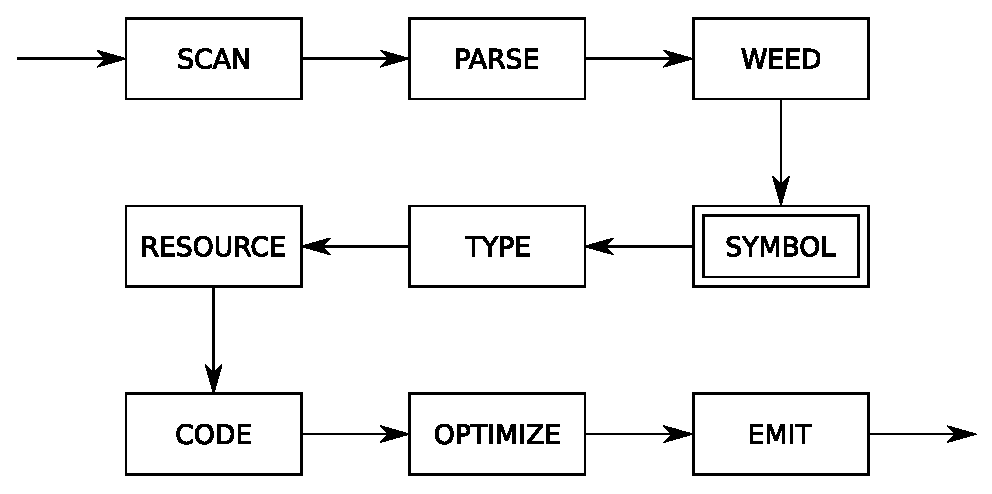
\psfig{file=figs/symbol.eps,width=20em}
\end{center}

\vfil
\end{slide*}

\begin{slide*}
{\em Symbol tables\/} are used to describe and analyse
definitions and uses of identifiers.

Grammars are too weak; the language:
$$ \{w\alpha w | w \in \Sigma^*\} $$
is not context-free.

A symbol table is a map from identifiers to meanings:

\begin{scriptsize}
\begin{center}
\begin{tabular}{|l|l|l|}
\hline
{\tt i} & local & int \\\hline
{\tt done} & local & boolean\\\hline
{\tt insert} & method & \ldots\\\hline
{\tt List} & class & \ldots\\\hline
{\tt x} & formal & {\tt List}\\\hline
 $\vdots$ & $\vdots$ & $\vdots$\\
\end{tabular}
\end{center}
\end{scriptsize}

We must construct a symbol table for every program point.
\vfil
\end{slide*}
 
\begin{slide*}
Using symbol tables to analyse JOOS:

\begin{itemize}
\item which classes are defined;
\item what is the inheritance hierarchy;
\item is the hierarchy well-formed;
\item which fields are defined;
\item which methods are defined;
\item what are the signatures of methods;
\item are identifiers defined twice;
\item are identifiers defined when used; and
\item are identifiers used properly?
\end{itemize}
\vfil
\end{slide*}
 
\begin{slide*}
Static, nested scope rules:
\vspace*{1em}

\setlength{\unitlength}{0.000400in}%
%
\begingroup\makeatletter\ifx\SetFigFont\undefined%
\gdef\SetFigFont#1#2#3#4#5{%
  \reset@font\fontsize{#1}{#2pt}%
  \fontfamily{#3}\fontseries{#4}\fontshape{#5}%
  \selectfont}%
\fi\endgroup%
\begin{picture}(7149,6924)(1189,-7273)
\thicklines
\put(1201,-7261){\framebox(4800,6900){}}
\put(1801,-961){\framebox(3900,300){}}
\put(1801,-1561){\framebox(3900,300){}}
\put(1801,-6961){\framebox(3900,300){}}
\put(1801,-6361){\framebox(3900,4500){}}
\put(2401,-6061){\framebox(3000,1800){}}
\put(3001,-5161){\framebox(2100,600){}}
\put(3001,-5761){\framebox(2100,300){}}
\put(2401,-3961){\framebox(3000,1800){}}
\put(3001,-3661){\framebox(2100,1200){}}
\put(3601,-3361){\framebox(1200,600){}}
\put(6976,-3886){\vector(-3,-1){2925}}
\put(6976,-3361){\line( 1, 0){1350}}
\put(6976,-3661){\line( 1, 0){1350}}
\put(6976,-3961){\line( 1, 0){1350}}
\put(6976,-4261){\line( 1, 0){1350}}
\put(6976,-4561){\line( 1, 0){1350}}
\put(6976,-4861){\line( 1, 0){1350}}
\put(6976,-5161){\line( 1, 0){1350}}
\put(6976,-5461){\framebox(1350,2400){}}
\put(7426,-3061){\line( 0,-1){2400}}
\put(1546,-886){\makebox(0,0)[lb]{\smash{\SetFigFont{8}{14.4}{\familydefault}{\mddefault}{\updefault}A}}}
\put(1546,-1486){\makebox(0,0)[lb]{\smash{\SetFigFont{8}{14.4}{\familydefault}{\mddefault}{\updefault}B}}}
\put(1546,-2086){\makebox(0,0)[lb]{\smash{\SetFigFont{8}{14.4}{\familydefault}{\mddefault}{\updefault}C}}}
\put(2146,-2386){\makebox(0,0)[lb]{\smash{\SetFigFont{8}{14.4}{\familydefault}{\mddefault}{\updefault}E}}}
\put(2746,-2686){\makebox(0,0)[lb]{\smash{\SetFigFont{8}{14.4}{\familydefault}{\mddefault}{\updefault}G}}}
\put(3346,-2986){\makebox(0,0)[lb]{\smash{\SetFigFont{8}{14.4}{\familydefault}{\mddefault}{\updefault}H}}}
\put(2821,-4786){\makebox(0,0)[lb]{\smash{\SetFigFont{8}{14.4}{\familydefault}{\mddefault}{\updefault}I}}}
\put(2146,-4486){\makebox(0,0)[lb]{\smash{\SetFigFont{8}{14.4}{\familydefault}{\mddefault}{\updefault}F}}}
\put(2821,-5686){\makebox(0,0)[lb]{\smash{\SetFigFont{8}{14.4}{\familydefault}{\mddefault}{\updefault}J}}}
\put(1546,-6886){\makebox(0,0)[lb]{\smash{\SetFigFont{8}{14.4}{\familydefault}{\mddefault}{\updefault}D}}}
\put(7126,-3286){\makebox(0,0)[lb]{\smash{\SetFigFont{8}{14.4}{\familydefault}{\mddefault}{\updefault}A}}}
\put(7126,-3586){\makebox(0,0)[lb]{\smash{\SetFigFont{8}{14.4}{\familydefault}{\mddefault}{\updefault}B}}}
\put(7126,-3886){\makebox(0,0)[lb]{\smash{\SetFigFont{8}{14.4}{\familydefault}{\mddefault}{\updefault}C}}}
\put(7126,-4186){\makebox(0,0)[lb]{\smash{\SetFigFont{8}{14.4}{\familydefault}{\mddefault}{\updefault}D}}}
\put(7126,-4486){\makebox(0,0)[lb]{\smash{\SetFigFont{8}{14.4}{\familydefault}{\mddefault}{\updefault}E}}}
\put(7126,-4786){\makebox(0,0)[lb]{\smash{\SetFigFont{8}{14.4}{\familydefault}{\mddefault}{\updefault}F}}}
\put(7126,-5086){\makebox(0,0)[lb]{\smash{\SetFigFont{8}{14.4}{\familydefault}{\mddefault}{\updefault}I}}}
\put(7126,-5386){\makebox(0,0)[lb]{\smash{\SetFigFont{8}{14.4}{\familydefault}{\mddefault}{\updefault}J}}}
\put(6801,-5750){\makebox(0,0)[lb]{\smash{\SetFigFont{8}{14.4}{\familydefault}{\mddefault}{\updefault}symbol table}}}
\end{picture}

The standard of modern languages.
\vfil
\end{slide*}
 
\begin{slide*}
Old-style one-pass technology:
\vspace*{1em}

\setlength{\unitlength}{0.000400in}%
%
\begingroup\makeatletter\ifx\SetFigFont\undefined%
\gdef\SetFigFont#1#2#3#4#5{%
  \reset@font\fontsize{#1}{#2pt}%
  \fontfamily{#3}\fontseries{#4}\fontshape{#5}%
  \selectfont}%
\fi\endgroup%
\begin{picture}(7149,6924)(1189,-7273)
\thicklines
\put(1201,-7261){\framebox(4800,6900){}}
\put(1801,-961){\framebox(3900,300){}}
\put(1801,-1561){\framebox(3900,300){}}
\put(1801,-6961){\framebox(3900,300){}}
\put(1801,-6361){\framebox(3900,4500){}}
\put(2401,-6061){\framebox(3000,1800){}}
\put(3001,-5161){\framebox(2100,600){}}
\put(3001,-5761){\framebox(2100,300){}}
\put(2401,-3961){\framebox(3000,1800){}}
\put(3001,-3661){\framebox(2100,1200){}}
\put(3601,-3361){\framebox(1200,600){}}
\put(6976,-3886){\vector(-3,-1){2925}}
\put(6976,-3361){\line( 1, 0){1350}}
\put(6976,-3661){\line( 1, 0){1350}}
\put(6976,-3961){\line( 1, 0){1350}}
\put(6976,-4261){\line( 1, 0){1350}}
\put(6976,-4561){\line( 1, 0){1350}}
\put(6976,-4861){\line( 1, 0){1350}}
\put(6976,-5161){\line( 1, 0){1350}}
\put(6976,-5461){\framebox(1350,2400){}}
\put(7426,-3061){\line( 0,-1){2400}}
\put(6749,-3973){\line( 6,-1){1800}}
\put(6751,-4261){\line( 6, 1){1800}}
\put(6751,-5461){\line( 6, 1){1800}}
\put(6751,-5161){\line( 6,-1){1800}}
\put(1546,-886){\makebox(0,0)[lb]{\smash{\SetFigFont{8}{14.4}{\familydefault}{\mddefault}{\updefault}A}}}
\put(1546,-1486){\makebox(0,0)[lb]{\smash{\SetFigFont{8}{14.4}{\familydefault}{\mddefault}{\updefault}B}}}
\put(1546,-2086){\makebox(0,0)[lb]{\smash{\SetFigFont{8}{14.4}{\familydefault}{\mddefault}{\updefault}C}}}
\put(2146,-2386){\makebox(0,0)[lb]{\smash{\SetFigFont{8}{14.4}{\familydefault}{\mddefault}{\updefault}E}}}
\put(2746,-2686){\makebox(0,0)[lb]{\smash{\SetFigFont{8}{14.4}{\familydefault}{\mddefault}{\updefault}G}}}
\put(3346,-2986){\makebox(0,0)[lb]{\smash{\SetFigFont{8}{14.4}{\familydefault}{\mddefault}{\updefault}H}}}
\put(2821,-4786){\makebox(0,0)[lb]{\smash{\SetFigFont{8}{14.4}{\familydefault}{\mddefault}{\updefault}I}}}
\put(2146,-4486){\makebox(0,0)[lb]{\smash{\SetFigFont{8}{14.4}{\familydefault}{\mddefault}{\updefault}F}}}
\put(2821,-5686){\makebox(0,0)[lb]{\smash{\SetFigFont{8}{14.4}{\familydefault}{\mddefault}{\updefault}J}}}
\put(1546,-6886){\makebox(0,0)[lb]{\smash{\SetFigFont{8}{14.4}{\familydefault}{\mddefault}{\updefault}D}}}
\put(7126,-3286){\makebox(0,0)[lb]{\smash{\SetFigFont{8}{14.4}{\familydefault}{\mddefault}{\updefault}A}}}
\put(7126,-3586){\makebox(0,0)[lb]{\smash{\SetFigFont{8}{14.4}{\familydefault}{\mddefault}{\updefault}B}}}
\put(7126,-3886){\makebox(0,0)[lb]{\smash{\SetFigFont{8}{14.4}{\familydefault}{\mddefault}{\updefault}C}}}
\put(7126,-4186){\makebox(0,0)[lb]{\smash{\SetFigFont{8}{14.4}{\familydefault}{\mddefault}{\updefault}D}}}
\put(7126,-4486){\makebox(0,0)[lb]{\smash{\SetFigFont{8}{14.4}{\familydefault}{\mddefault}{\updefault}E}}}
\put(7126,-4786){\makebox(0,0)[lb]{\smash{\SetFigFont{8}{14.4}{\familydefault}{\mddefault}{\updefault}F}}}
\put(7126,-5086){\makebox(0,0)[lb]{\smash{\SetFigFont{8}{14.4}{\familydefault}{\mddefault}{\updefault}I}}}
\put(7126,-5386){\makebox(0,0)[lb]{\smash{\SetFigFont{8}{14.4}{\familydefault}{\mddefault}{\updefault}J}}}
\put(6801,-5750){\makebox(0,0)[lb]{\smash{\SetFigFont{8}{14.4}{\familydefault}{\mddefault}{\updefault}symbol table}}}
\end{picture}
\vfil
Still haunts some languages:
\begin{scriptsize}
\begin{verbatim}
void weedPROGRAM(PROGRAM *p);
void weedCLASSFILE(CLASSFILE *c);
void weedCLASS(CLASS *c);
\end{verbatim}
\end{scriptsize}
Forward declarations enable recursion.
\vfil
\end{slide*}
 
\begin{slide*}
Use the most closely nested definition:
\vspace*{1em}

\setlength{\unitlength}{0.000400in}%
%
\begingroup\makeatletter\ifx\SetFigFont\undefined%
\gdef\SetFigFont#1#2#3#4#5{%
  \reset@font\fontsize{#1}{#2pt}%
  \fontfamily{#3}\fontseries{#4}\fontshape{#5}%
  \selectfont}%
\fi\endgroup%
\begin{picture}(7149,6924)(1189,-7273)
\thicklines
\put(1201,-7261){\framebox(4800,6900){}}
\put(1801,-961){\framebox(3900,300){}}
\put(1801,-1561){\framebox(3900,300){}}
\put(1801,-6961){\framebox(3900,300){}}
\put(1801,-6361){\framebox(3900,4500){}}
\put(2401,-6061){\framebox(3000,1800){}}
\put(3001,-5161){\framebox(2100,600){}}
\put(3001,-5761){\framebox(2100,300){}}
\put(2401,-3961){\framebox(3000,1800){}}
\put(3001,-3661){\framebox(2100,1200){}}
\put(3601,-3361){\framebox(1200,600){}}
\put(6976,-3886){\vector(-3,-1){2925}}
\put(6976,-3361){\line( 1, 0){1350}}
\put(6976,-3661){\line( 1, 0){1350}}
\put(6976,-3961){\line( 1, 0){1350}}
\put(6976,-4261){\line( 1, 0){1350}}
\put(6976,-4561){\line( 1, 0){1350}}
\put(6976,-4861){\framebox(1350,1800){}}
\put(7426,-3061){\line( 0,-1){1800}}
\put(1456,-886){\makebox(0,0)[lb]{\smash{\SetFigFont{8}{14.4}{\familydefault}{\mddefault}{\updefault}A$_1$}}}
\put(1546,-1486){\makebox(0,0)[lb]{\smash{\SetFigFont{8}{14.4}{\familydefault}{\mddefault}{\updefault}B}}}
\put(1546,-2086){\makebox(0,0)[lb]{\smash{\SetFigFont{8}{14.4}{\familydefault}{\mddefault}{\updefault}C}}}
\put(2746,-2686){\makebox(0,0)[lb]{\smash{\SetFigFont{8}{14.4}{\familydefault}{\mddefault}{\updefault}G}}}
\put(3346,-2986){\makebox(0,0)[lb]{\smash{\SetFigFont{8}{14.4}{\familydefault}{\mddefault}{\updefault}H}}}
\put(2821,-4786){\makebox(0,0)[lb]{\smash{\SetFigFont{8}{14.4}{\familydefault}{\mddefault}{\updefault}I}}}
\put(2146,-4486){\makebox(0,0)[lb]{\smash{\SetFigFont{8}{14.4}{\familydefault}{\mddefault}{\updefault}F}}}
\put(1546,-6886){\makebox(0,0)[lb]{\smash{\SetFigFont{8}{14.4}{\familydefault}{\mddefault}{\updefault}D}}}
\put(7126,-3586){\makebox(0,0)[lb]{\smash{\SetFigFont{8}{14.4}{\familydefault}{\mddefault}{\updefault}B}}}
\put(7126,-3886){\makebox(0,0)[lb]{\smash{\SetFigFont{8}{14.4}{\familydefault}{\mddefault}{\updefault}C}}}
\put(7126,-4186){\makebox(0,0)[lb]{\smash{\SetFigFont{8}{14.4}{\familydefault}{\mddefault}{\updefault}D}}}
\put(2056,-2386){\makebox(0,0)[lb]{\smash{\SetFigFont{8}{14.4}{\familydefault}{\mddefault}{\updefault}A$_2$}}}
\put(2676,-5686){\makebox(0,0)[lb]{\smash{\SetFigFont{8}{14.4}{\rmdefault}{\mddefault}{\updefault}A$_3$}}}
\put(7056,-3286){\makebox(0,0)[lb]{\smash{\SetFigFont{8}{14.4}{\familydefault}{\mddefault}{\updefault}A$_3$}}}
\put(7126,-4486){\makebox(0,0)[lb]{\smash{\SetFigFont{8}{14.4}{\familydefault}{\mddefault}{\updefault}F}}}
\put(7126,-4786){\makebox(0,0)[lb]{\smash{\SetFigFont{8}{14.4}{\familydefault}{\mddefault}{\updefault}I}}}
\put(6801,-5150){\makebox(0,0)[lb]{\smash{\SetFigFont{8}{14.4}{\familydefault}{\mddefault}{\updefault}symbol table}}}
\end{picture}

Identifiers at same level must be unique.
\vfil
\end{slide*}
 
\begin{slide*}
The symbol table behaves like a stack:
\vspace*{1em}

\setlength{\unitlength}{0.000400in}%
%
\begingroup\makeatletter\ifx\SetFigFont\undefined%
\gdef\SetFigFont#1#2#3#4#5{%
  \reset@font\fontsize{#1}{#2pt}%
  \fontfamily{#3}\fontseries{#4}\fontshape{#5}%
  \selectfont}%
\fi\endgroup%
\begin{picture}(5424,6924)(1189,-7273)
\thicklines
\put(1201,-7261){\framebox(4800,6900){}}
\put(1801,-961){\framebox(3900,300){}}
\put(1801,-1561){\framebox(3900,300){}}
\put(1801,-6961){\framebox(3900,300){}}
\put(1801,-6361){\framebox(3900,4500){}}
\put(2401,-6061){\framebox(3000,1800){}}
\put(3001,-5161){\framebox(2100,600){}}
\put(3001,-5761){\framebox(2100,300){}}
\put(2401,-3961){\framebox(3000,1800){}}
\put(3001,-3661){\framebox(2100,1200){}}
\put(3601,-3361){\framebox(1200,600){}}
\put(6601,-1111){\vector(-1, 0){1800}}
\put(6601,-2011){\vector(-1, 0){1800}}
\put(6601,-2311){\vector(-1, 0){1800}}
\put(6601,-2611){\vector(-1, 0){1800}}
\put(6601,-4111){\vector(-1, 0){1800}}
\put(6601,-3811){\vector(-1, 0){1800}}
\put(6601,-4411){\vector(-1, 0){1800}}
\put(6601,-6211){\vector(-1, 0){1800}}
\put(6601,-6511){\vector(-1, 0){1800}}
\put(1546,-886){\makebox(0,0)[lb]{\smash{\SetFigFont{8}{14.4}{\familydefault}{\mddefault}{\updefault}A}}}
\put(1546,-1486){\makebox(0,0)[lb]{\smash{\SetFigFont{8}{14.4}{\familydefault}{\mddefault}{\updefault}B}}}
\put(1546,-2086){\makebox(0,0)[lb]{\smash{\SetFigFont{8}{14.4}{\familydefault}{\mddefault}{\updefault}C}}}
\put(2146,-2386){\makebox(0,0)[lb]{\smash{\SetFigFont{8}{14.4}{\familydefault}{\mddefault}{\updefault}E}}}
\put(2746,-2686){\makebox(0,0)[lb]{\smash{\SetFigFont{8}{14.4}{\familydefault}{\mddefault}{\updefault}G}}}
\put(3346,-2986){\makebox(0,0)[lb]{\smash{\SetFigFont{8}{14.4}{\familydefault}{\mddefault}{\updefault}H}}}
\put(2831,-4786){\makebox(0,0)[lb]{\smash{\SetFigFont{8}{14.4}{\familydefault}{\mddefault}{\updefault}I}}}
\put(2146,-4486){\makebox(0,0)[lb]{\smash{\SetFigFont{8}{14.4}{\familydefault}{\mddefault}{\updefault}F}}}
\put(2821,-5686){\makebox(0,0)[lb]{\smash{\SetFigFont{8}{14.4}{\familydefault}{\mddefault}{\updefault}J}}}
\put(1546,-6886){\makebox(0,0)[lb]{\smash{\SetFigFont{8}{14.4}{\familydefault}{\mddefault}{\updefault}D}}}
\put(6601,-1186){\makebox(0,0)[lb]{\smash{\SetFigFont{8}{14.4}{\rmdefault}{\mddefault}{\updefault}ABCD}}}
\put(6601,-2086){\makebox(0,0)[lb]{\smash{\SetFigFont{8}{14.4}{\rmdefault}{\mddefault}{\updefault}ABCD$|$EF}}}
\put(6601,-2386){\makebox(0,0)[lb]{\smash{\SetFigFont{8}{14.4}{\rmdefault}{\mddefault}{\updefault}ABCD$|$EF$|$G}}}
\put(6601,-2686){\makebox(0,0)[lb]{\smash{\SetFigFont{8}{14.4}{\rmdefault}{\mddefault}{\updefault}ABCD$|$EF$|$G$|$H}}}
\put(6601,-4186){\makebox(0,0)[lb]{\smash{\SetFigFont{8}{14.4}{\rmdefault}{\mddefault}{\updefault}ABCD$|$EF}}}
\put(6601,-4486){\makebox(0,0)[lb]{\smash{\SetFigFont{8}{14.4}{\rmdefault}{\mddefault}{\updefault}ABCD$|$EF$|$IJ}}}
\put(6601,-6586){\makebox(0,0)[lb]{\smash{\SetFigFont{8}{14.4}{\rmdefault}{\mddefault}{\updefault}ABCD}}}
\put(6601,-3886){\makebox(0,0)[lb]{\smash{\SetFigFont{8}{14.4}{\rmdefault}{\mddefault}{\updefault}ABCD$|$EF$|$G}}}
\put(6601,-6286){\makebox(0,0)[lb]{\smash{\SetFigFont{8}{14.4}{\rmdefault}{\mddefault}{\updefault}ABCD$|$EF}}}
\end{picture}
\vfil
\end{slide*}
 
\begin{slide*}
The symbol table can be implemented as a simple stack:

\begin{scriptsize}
\begin{itemize}
\item {\tt pushSymbol(SymbolTable *t, char *name, ...)}
\item {\tt popSymbol(SymbolTable *t)}
\item {\tt getSymbol(SymbolTable *t, char *name)}
\end{itemize}
\end{scriptsize}

But how do we detect multiple definitions of an identifier at the same level?

Use {\em bookmarks} and a {\em cactus stack}:

\begin{scriptsize}
\begin{itemize}
\item {\tt scopeSymbolTable(SymbolTable *t)}
\item {\tt putSymbol(SymbolTable *t, char *name, ...)}
\item {\tt unscopeSymbolTable(SymbolTable *t)}
\item {\tt getSymbol(SymbolTable *t, char *name)}
\end{itemize}
\end{scriptsize}

Still just linear search, though.

\vfil
\end{slide*}
 
\begin{slide*}
Implement symbol tables as a cactus stack of {\em hash tables}:

\begin{itemize}
\item each hash table contains the identifiers in a level;

\item push a new hash table when a level is entered;

\item each identifier is entered in the top hash table;

\item it is an error if it is already there;

\item a use of an identifier is looked up in the hash tables from top to bottom;

\item it is an error if it is not found;

\item pop a hash table when a level is left.
\end{itemize}
\vfil
\end{slide*}

\begin{slide*}
What is a good hash function on identifiers?
 
Use the initial letter:
\begin{itemize}
\item {\tt codePROGRAM}, {\tt codeMETHOD}, {\tt codeEXP}, \ldots
\end{itemize}

Use the sum of the letters:
\begin{itemize}
\item doesn't distinguish letter order
\end{itemize}

Use the shifted sum of the letters:
{\tt
\begin{tabbing}
~~"j" \= = 106 = \=0000000001101010\\
shift      \>\>0000000011010100\\
+ "o" \> = 111 = \>0000000001101111\\
=           \>\>0000000101000011\\
shift \>\>0000001010000110\\
+ "o" \> = 111 = \>0000000001101111\\
=           \>\>0000001011110101\\
shift\>\>0000010111101010\\
+ "s" \> = 115 = \>0000000001110011\\
= \>\>0000011001011101\\
= \>\>1629
\end{tabbing}
}

\vfil
\end{slide*}

\begin{slide*}
Hash tables for the JOOS source code:\\
~\\
\begin{barenv}
\setlength{\unitlength}{0.6pt}
\setnumberpos{empty}
\setstretch{1.2}
\setwidth{1}
\bar{0}{8}
\bar{0}{8}
\bar{0}{8}
\bar{0}{8}
\bar{0}{8}
\bar{0}{8}
\bar{0}{8}
\bar{0}{8}
\bar{0}{8}
\bar{0}{8}
\bar{0}{8}
\bar{0}{8}
\bar{0}{8}
\bar{0}{8}
\bar{0}{8}
\bar{0}{8}
\bar{0}{8}
\bar{0}{8}
\bar{0}{8}
\bar{0}{8}
\bar{0}{8}
\bar{0}{8}
\bar{0}{8}
\bar{0}{8}
\bar{0}{8}
\bar{0}{8}
\bar{0}{8}
\bar{0}{8}
\bar{0}{8}
\bar{0}{8}
\bar{0}{8}
\bar{0}{8}
\bar{0}{8}
\bar{0}{8}
\bar{0}{8}
\bar{0}{8}
\bar{0}{8}
\bar{0}{8}
\bar{0}{8}
\bar{0}{8}
\bar{0}{8}
\bar{0}{8}
\bar{0}{8}
\bar{0}{8}
\bar{0}{8}
\bar{0}{8}
\bar{0}{8}
\bar{0}{8}
\bar{0}{8}
\bar{0}{8}
\bar{0}{8}
\bar{0}{8}
\bar{0}{8}
\bar{0}{8}
\bar{0}{8}
\bar{0}{8}
\bar{0}{8}
\bar{0}{8}
\bar{0}{8}
\bar{0}{8}
\bar{0}{8}
\bar{0}{8}
\bar{0}{8}
\bar{0}{8}
\bar{0}{8}
\bar{8}{8}
\bar{4}{8}
\bar{15}{8}
\bar{7}{8}
\bar{14}{8}
\bar{12}{8}
\bar{7}{8}
\bar{4}{8}
\bar{12}{8}
\bar{1}{8}
\bar{0}{8}
\bar{5}{8}
\bar{8}{8}
\bar{11}{8}
\bar{7}{8}
\bar{11}{8}
\bar{0}{8}
\bar{13}{8}
\bar{20}{8}
\bar{7}{8}
\bar{4}{8}
\bar{1}{8}
\bar{7}{8}
\bar{1}{8}
\bar{85}{8}
\bar{1}{8}
\bar{0}{8}
\bar{0}{8}
\bar{0}{8}
\bar{0}{8}
\bar{13}{8}
\bar{0}{8}
\bar{73}{8}
\bar{38}{8}
\bar{144}{8}
\bar{47}{8}
\bar{71}{8}
\bar{58}{8}
\bar{28}{8}
\bar{20}{8}
\bar{187}{8}
\bar{6}{8}
\bar{6}{8}
\bar{62}{8}
\bar{142}{8}
\bar{46}{8}
\bar{46}{8}
\bar{63}{8}
\bar{0}{8}
\bar{77}{8}
\bar{184}{8}
\bar{143}{8}
\bar{34}{8}
\bar{15}{8}
\bar{41}{8}
\bar{1}{8}
\bar{139}{8}
\bar{0}{8}
\bar{0}{8}
\bar{0}{8}
\bar{0}{8}
\bar{0}{8}
\bar{0}{8}
\bar{0}{8}
\bar{0}{8}
\bar{0}{8}
\bar{0}{8}
\bar{0}{8}
\bar{0}{8}
\bar{0}{8}
\bar{0}{8}
\bar{0}{8}
\bar{0}{8}
\bar{0}{8}
\bar{0}{8}
\bar{0}{8}
\bar{0}{8}
\bar{0}{8}
\bar{0}{8}
\bar{0}{8}
\bar{0}{8}
\bar{0}{8}
\bar{0}{8}
\bar{0}{8}
\bar{0}{8}
\bar{0}{8}
\bar{0}{8}
\bar{0}{8}
\bar{0}{8}
\bar{0}{8}
\bar{0}{8}
\bar{0}{8}
\bar{0}{8}
\bar{0}{8}
\bar{0}{8}
\bar{0}{8}
\bar{0}{8}
\bar{0}{8}
\bar{0}{8}
\bar{0}{8}
\bar{0}{8}
\bar{0}{8}
\bar{0}{8}
\bar{0}{8}
\bar{0}{8}
\bar{0}{8}
\bar{0}{8}
\bar{0}{8}
\bar{0}{8}
\bar{0}{8}
\bar{0}{8}
\bar{0}{8}
\bar{0}{8}
\bar{0}{8}
\bar{0}{8}
\bar{0}{8}
\bar{0}{8}
\bar{0}{8}
\bar{0}{8}
\bar{0}{8}
\bar{0}{8}
\bar{0}{8}
\bar{0}{8}
\bar{0}{8}
\bar{0}{8}
\bar{0}{8}
\bar{0}{8}
\bar{0}{8}
\bar{0}{8}
\bar{0}{8}
\bar{0}{8}
\bar{0}{8}
\bar{0}{8}
\bar{0}{8}
\bar{0}{8}
\bar{0}{8}
\bar{0}{8}
\bar{0}{8}
\bar{0}{8}
\bar{0}{8}
\bar{0}{8}
\bar{0}{8}
\bar{0}{8}
\bar{0}{8}
\bar{0}{8}
\bar{0}{8}
\bar{0}{8}
\bar{0}{8}
\bar{0}{8}
\bar{0}{8}
\bar{0}{8}
\bar{0}{8}
\bar{0}{8}
\bar{0}{8}
\bar{0}{8}
\bar{0}{8}
\bar{0}{8}
\bar{0}{8}
\bar{0}{8}
\bar{0}{8}
\bar{0}{8}
\bar{0}{8}
\bar{0}{8}
\bar{0}{8}
\bar{0}{8}
\bar{0}{8}
\bar{0}{8}
\bar{0}{8}
\bar{0}{8}
\bar{0}{8}
\bar{0}{8}
\bar{0}{8}
\bar{0}{8}
\bar{0}{8}
\bar{0}{8}
\bar{0}{8}
\bar{0}{8}
\bar{0}{8}
\bar{0}{8}
\bar{0}{8}
\bar{0}{8}
\bar{0}{8}
\bar{0}{8}
\bar{0}{8}
\bar{0}{8}
\bar{0}{8}
\bar{0}{8}
\bar{0}{8}
\bar{0}{8}
\bar{0}{8}
\bar{0}{8}
\bar{0}{8}
\bar{0}{8}
\bar{0}{8}
\bar{0}{8}
\bar{0}{8}
\bar{0}{8}
\bar{0}{8}
\bar{0}{8}
\bar{0}{8}
\bar{0}{8}
\bar{0}{8}
\bar{0}{8}
\bar{0}{8}
\bar{0}{8}
\bar{0}{8}
\bar{0}{8}
\bar{0}{8}
\bar{0}{8}
\bar{0}{8}
\bar{0}{8}
\bar{0}{8}
\bar{0}{8}
\bar{0}{8}
\bar{0}{8}
\bar{0}{8}
\bar{0}{8}
\bar{0}{8}
\bar{0}{8}
\bar{0}{8}
\bar{0}{8}
\bar{0}{8}
\bar{0}{8}
\bar{0}{8}
\bar{0}{8}
\bar{0}{8}
\bar{0}{8}
\bar{0}{8}
\bar{0}{8}
\bar{0}{8}
\bar{0}{8}
\bar{0}{8}
\bar{0}{8}
\bar{0}{8}
\bar{0}{8}
\bar{0}{8}
\bar{0}{8}
\bar{0}{8}
\bar{0}{8}
\bar{0}{8}
\bar{0}{8}
\bar{0}{8}
\bar{0}{8}
\bar{0}{8}
\bar{0}{8}
\bar{0}{8}
\bar{0}{8}
\bar{0}{8}
\bar{0}{8}
\bar{0}{8}
\bar{0}{8}
\bar{0}{8}
\end{barenv}
\mbox{}\hfil{\scriptsize \verb"hash = *str;"}\hfil
\vfil
\end{slide*}

\begin{slide*}
Hash tables for the JOOS source code:\\
~\\
\begin{barenv}
\setlength{\unitlength}{0.6pt}
\setnumberpos{empty}
\setstretch{5}
\setwidth{1}
\bar{13}{8}
\bar{5}{8}
\bar{10}{8}
\bar{10}{8}
\bar{10}{8}
\bar{5}{8}
\bar{7}{8}
\bar{6}{8}
\bar{8}{8}
\bar{8}{8}
\bar{11}{8}
\bar{10}{8}
\bar{4}{8}
\bar{15}{8}
\bar{13}{8}
\bar{17}{8}
\bar{17}{8}
\bar{4}{8}
\bar{10}{8}
\bar{7}{8}
\bar{10}{8}
\bar{12}{8}
\bar{7}{8}
\bar{13}{8}
\bar{6}{8}
\bar{6}{8}
\bar{10}{8}
\bar{6}{8}
\bar{10}{8}
\bar{7}{8}
\bar{7}{8}
\bar{8}{8}
\bar{4}{8}
\bar{6}{8}
\bar{10}{8}
\bar{10}{8}
\bar{5}{8}
\bar{5}{8}
\bar{2}{8}
\bar{5}{8}
\bar{4}{8}
\bar{4}{8}
\bar{3}{8}
\bar{5}{8}
\bar{6}{8}
\bar{7}{8}
\bar{4}{8}
\bar{5}{8}
\bar{6}{8}
\bar{4}{8}
\bar{3}{8}
\bar{1}{8}
\bar{4}{8}
\bar{5}{8}
\bar{3}{8}
\bar{3}{8}
\bar{1}{8}
\bar{5}{8}
\bar{2}{8}
\bar{4}{8}
\bar{2}{8}
\bar{3}{8}
\bar{4}{8}
\bar{2}{8}
\bar{3}{8}
\bar{5}{8}
\bar{3}{8}
\bar{5}{8}
\bar{3}{8}
\bar{4}{8}
\bar{3}{8}
\bar{7}{8}
\bar{5}{8}
\bar{6}{8}
\bar{6}{8}
\bar{6}{8}
\bar{7}{8}
\bar{2}{8}
\bar{5}{8}
\bar{7}{8}
\bar{5}{8}
\bar{4}{8}
\bar{4}{8}
\bar{5}{8}
\bar{5}{8}
\bar{7}{8}
\bar{3}{8}
\bar{5}{8}
\bar{3}{8}
\bar{8}{8}
\bar{6}{8}
\bar{4}{8}
\bar{2}{8}
\bar{11}{8}
\bar{8}{8}
\bar{8}{8}
\bar{8}{8}
\bar{7}{8}
\bar{6}{8}
\bar{8}{8}
\bar{8}{8}
\bar{8}{8}
\bar{8}{8}
\bar{10}{8}
\bar{12}{8}
\bar{11}{8}
\bar{6}{8}
\bar{8}{8}
\bar{13}{8}
\bar{5}{8}
\bar{13}{8}
\bar{7}{8}
\bar{11}{8}
\bar{9}{8}
\bar{14}{8}
\bar{10}{8}
\bar{9}{8}
\bar{8}{8}
\bar{13}{8}
\bar{14}{8}
\bar{14}{8}
\bar{7}{8}
\bar{10}{8}
\bar{11}{8}
\bar{4}{8}
\bar{11}{8}
\bar{11}{8}
\bar{9}{8}
\bar{8}{8}
\bar{2}{8}
\bar{12}{8}
\bar{6}{8}
\bar{10}{8}
\bar{8}{8}
\bar{8}{8}
\bar{6}{8}
\bar{5}{8}
\bar{9}{8}
\bar{6}{8}
\bar{4}{8}
\bar{8}{8}
\bar{6}{8}
\bar{6}{8}
\bar{9}{8}
\bar{5}{8}
\bar{6}{8}
\bar{4}{8}
\bar{4}{8}
\bar{5}{8}
\bar{1}{8}
\bar{1}{8}
\bar{2}{8}
\bar{2}{8}
\bar{5}{8}
\bar{7}{8}
\bar{5}{8}
\bar{3}{8}
\bar{6}{8}
\bar{7}{8}
\bar{6}{8}
\bar{2}{8}
\bar{4}{8}
\bar{4}{8}
\bar{2}{8}
\bar{3}{8}
\bar{5}{8}
\bar{4}{8}
\bar{4}{8}
\bar{5}{8}
\bar{4}{8}
\bar{1}{8}
\bar{7}{8}
\bar{2}{8}
\bar{5}{8}
\bar{2}{8}
\bar{4}{8}
\bar{3}{8}
\bar{3}{8}
\bar{3}{8}
\bar{4}{8}
\bar{4}{8}
\bar{5}{8}
\bar{4}{8}
\bar{4}{8}
\bar{4}{8}
\bar{5}{8}
\bar{2}{8}
\bar{2}{8}
\bar{1}{8}
\bar{6}{8}
\bar{3}{8}
\bar{2}{8}
\bar{1}{8}
\bar{5}{8}
\bar{10}{8}
\bar{6}{8}
\bar{2}{8}
\bar{4}{8}
\bar{11}{8}
\bar{6}{8}
\bar{4}{8}
\bar{4}{8}
\bar{4}{8}
\bar{7}{8}
\bar{5}{8}
\bar{11}{8}
\bar{4}{8}
\bar{8}{8}
\bar{6}{8}
\bar{9}{8}
\bar{7}{8}
\bar{6}{8}
\bar{9}{8}
\bar{10}{8}
\bar{8}{8}
\bar{10}{8}
\bar{5}{8}
\bar{6}{8}
\bar{4}{8}
\bar{19}{8}
\bar{14}{8}
\bar{9}{8}
\bar{10}{8}
\bar{10}{8}
\bar{7}{8}
\bar{7}{8}
\bar{9}{8}
\bar{12}{8}
\bar{6}{8}
\bar{9}{8}
\bar{8}{8}
\bar{11}{8}
\bar{9}{8}
\bar{6}{8}
\bar{10}{8}
\bar{10}{8}
\bar{14}{8}
\bar{5}{8}
\bar{9}{8}
\bar{8}{8}
\bar{14}{8}
\bar{9}{8}
\bar{9}{8}
\bar{4}{8}
\bar{6}{8}
\bar{8}{8}
\bar{7}{8}
\bar{5}{8}
\bar{6}{8}
\bar{5}{8}
\bar{7}{8}
\bar{4}{8}
\bar{2}{8}
\bar{2}{8}
\bar{5}{8}
\bar{7}{8}
\bar{6}{8}
\bar{2}{8}
\bar{4}{8}
\bar{5}{8}
\bar{6}{8}
\bar{2}{8}
\bar{2}{8}
\bar{7}{8}
\bar{1}{8}
\bar{5}{8}
\bar{5}{8}
\bar{6}{8}
\bar{4}{8}
\bar{4}{8}
\bar{3}{8}
\bar{3}{8}
\bar{1}{8}
\bar{0}{8}
\bar{5}{8}
\bar{0}{8}
\bar{1}{8}
\bar{3}{8}
\bar{2}{8}
\bar{1}{8}
\bar{3}{8}
\bar{3}{8}
\bar{6}{8}
\bar{4}{8}
\bar{1}{8}
\bar{3}{8}
\bar{4}{8}
\bar{2}{8}
\bar{4}{8}
\bar{8}{8}
\bar{4}{8}
\bar{5}{8}
\bar{0}{8}
\bar{6}{8}
\bar{5}{8}
\bar{6}{8}
\bar{5}{8}
\bar{7}{8}
\bar{4}{8}
\bar{9}{8}
\bar{9}{8}
\bar{6}{8}
\bar{5}{8}
\bar{9}{8}
\bar{3}{8}
\bar{3}{8}
\bar{6}{8}
\bar{8}{8}
\bar{6}{8}
\bar{3}{8}
\bar{9}{8}
\bar{8}{8}
\bar{4}{8}
\bar{7}{8}
\bar{9}{8}
\bar{12}{8}
\bar{9}{8}
\end{barenv}
\mbox{}\hfil{\scriptsize \verb"while (*str) hash = hash + *str++;"}\hfil

~\\
\begin{barenv}
\setlength{\unitlength}{0.6pt}
\setnumberpos{empty}
\setstretch{5}
\setwidth{1}
\bar{12}{8}
\bar{13}{8}
\bar{9}{8}
\bar{6}{8}
\bar{10}{8}
\bar{6}{8}
\bar{5}{8}
\bar{10}{8}
\bar{5}{8}
\bar{1}{8}
\bar{7}{8}
\bar{6}{8}
\bar{5}{8}
\bar{11}{8}
\bar{8}{8}
\bar{5}{8}
\bar{6}{8}
\bar{10}{8}
\bar{6}{8}
\bar{7}{8}
\bar{4}{8}
\bar{5}{8}
\bar{11}{8}
\bar{9}{8}
\bar{7}{8}
\bar{11}{8}
\bar{7}{8}
\bar{3}{8}
\bar{7}{8}
\bar{6}{8}
\bar{10}{8}
\bar{4}{8}
\bar{3}{8}
\bar{10}{8}
\bar{6}{8}
\bar{5}{8}
\bar{4}{8}
\bar{3}{8}
\bar{6}{8}
\bar{4}{8}
\bar{4}{8}
\bar{4}{8}
\bar{2}{8}
\bar{5}{8}
\bar{5}{8}
\bar{10}{8}
\bar{11}{8}
\bar{7}{8}
\bar{3}{8}
\bar{6}{8}
\bar{3}{8}
\bar{6}{8}
\bar{4}{8}
\bar{2}{8}
\bar{8}{8}
\bar{6}{8}
\bar{2}{8}
\bar{8}{8}
\bar{3}{8}
\bar{10}{8}
\bar{8}{8}
\bar{5}{8}
\bar{7}{8}
\bar{9}{8}
\bar{6}{8}
\bar{7}{8}
\bar{8}{8}
\bar{1}{8}
\bar{6}{8}
\bar{7}{8}
\bar{7}{8}
\bar{6}{8}
\bar{7}{8}
\bar{6}{8}
\bar{6}{8}
\bar{6}{8}
\bar{3}{8}
\bar{6}{8}
\bar{4}{8}
\bar{6}{8}
\bar{7}{8}
\bar{6}{8}
\bar{9}{8}
\bar{5}{8}
\bar{5}{8}
\bar{8}{8}
\bar{10}{8}
\bar{9}{8}
\bar{4}{8}
\bar{2}{8}
\bar{6}{8}
\bar{4}{8}
\bar{5}{8}
\bar{8}{8}
\bar{11}{8}
\bar{13}{8}
\bar{7}{8}
\bar{6}{8}
\bar{10}{8}
\bar{5}{8}
\bar{4}{8}
\bar{10}{8}
\bar{12}{8}
\bar{7}{8}
\bar{6}{8}
\bar{9}{8}
\bar{7}{8}
\bar{7}{8}
\bar{9}{8}
\bar{6}{8}
\bar{6}{8}
\bar{6}{8}
\bar{14}{8}
\bar{7}{8}
\bar{7}{8}
\bar{6}{8}
\bar{9}{8}
\bar{9}{8}
\bar{4}{8}
\bar{8}{8}
\bar{9}{8}
\bar{5}{8}
\bar{9}{8}
\bar{6}{8}
\bar{5}{8}
\bar{2}{8}
\bar{6}{8}
\bar{5}{8}
\bar{3}{8}
\bar{8}{8}
\bar{6}{8}
\bar{11}{8}
\bar{6}{8}
\bar{6}{8}
\bar{8}{8}
\bar{12}{8}
\bar{4}{8}
\bar{4}{8}
\bar{5}{8}
\bar{3}{8}
\bar{9}{8}
\bar{2}{8}
\bar{2}{8}
\bar{8}{8}
\bar{12}{8}
\bar{9}{8}
\bar{7}{8}
\bar{7}{8}
\bar{4}{8}
\bar{5}{8}
\bar{7}{8}
\bar{5}{8}
\bar{10}{8}
\bar{5}{8}
\bar{6}{8}
\bar{3}{8}
\bar{8}{8}
\bar{3}{8}
\bar{10}{8}
\bar{6}{8}
\bar{12}{8}
\bar{8}{8}
\bar{5}{8}
\bar{5}{8}
\bar{2}{8}
\bar{5}{8}
\bar{8}{8}
\bar{7}{8}
\bar{6}{8}
\bar{5}{8}
\bar{1}{8}
\bar{8}{8}
\bar{8}{8}
\bar{7}{8}
\bar{5}{8}
\bar{9}{8}
\bar{3}{8}
\bar{3}{8}
\bar{6}{8}
\bar{5}{8}
\bar{5}{8}
\bar{8}{8}
\bar{3}{8}
\bar{6}{8}
\bar{3}{8}
\bar{7}{8}
\bar{4}{8}
\bar{7}{8}
\bar{6}{8}
\bar{5}{8}
\bar{4}{8}
\bar{7}{8}
\bar{8}{8}
\bar{3}{8}
\bar{3}{8}
\bar{7}{8}
\bar{5}{8}
\bar{4}{8}
\bar{5}{8}
\bar{4}{8}
\bar{4}{8}
\bar{4}{8}
\bar{4}{8}
\bar{5}{8}
\bar{8}{8}
\bar{3}{8}
\bar{4}{8}
\bar{3}{8}
\bar{8}{8}
\bar{4}{8}
\bar{1}{8}
\bar{3}{8}
\bar{7}{8}
\bar{5}{8}
\bar{4}{8}
\bar{4}{8}
\bar{3}{8}
\bar{5}{8}
\bar{7}{8}
\bar{11}{8}
\bar{1}{8}
\bar{4}{8}
\bar{9}{8}
\bar{5}{8}
\bar{6}{8}
\bar{5}{8}
\bar{4}{8}
\bar{3}{8}
\bar{11}{8}
\bar{4}{8}
\bar{10}{8}
\bar{7}{8}
\bar{5}{8}
\bar{4}{8}
\bar{5}{8}
\bar{4}{8}
\bar{9}{8}
\bar{4}{8}
\bar{9}{8}
\bar{5}{8}
\bar{3}{8}
\bar{8}{8}
\bar{11}{8}
\bar{2}{8}
\bar{9}{8}
\bar{6}{8}
\bar{5}{8}
\bar{6}{8}
\bar{3}{8}
\bar{7}{8}
\bar{10}{8}
\bar{5}{8}
\bar{3}{8}
\bar{7}{8}
\bar{5}{8}
\bar{2}{8}
\bar{11}{8}
\bar{5}{8}
\bar{1}{8}
\bar{7}{8}
\bar{5}{8}
\bar{7}{8}
\bar{6}{8}
\bar{10}{8}
\bar{2}{8}
\bar{6}{8}
\bar{7}{8}
\bar{9}{8}
\bar{7}{8}
\bar{10}{8}
\bar{3}{8}
\bar{4}{8}
\bar{8}{8}
\bar{5}{8}
\bar{4}{8}
\bar{4}{8}
\bar{3}{8}
\bar{9}{8}
\bar{2}{8}
\bar{3}{8}
\bar{2}{8}
\bar{8}{8}
\bar{10}{8}
\bar{3}{8}
\bar{7}{8}
\bar{8}{8}
\bar{3}{8}
\bar{7}{8}
\bar{7}{8}
\bar{1}{8}
\bar{4}{8}
\bar{9}{8}
\bar{7}{8}
\bar{4}{8}
\bar{7}{8}
\bar{8}{8}
\bar{9}{8}
\bar{13}{8}
\bar{6}{8}
\bar{3}{8}
\bar{5}{8}
\bar{11}{8}
\bar{4}{8}
\bar{4}{8}
\bar{7}{8}
\bar{7}{8}
\bar{10}{8}
\bar{10}{8}
\bar{4}{8}
\bar{6}{8}
\bar{6}{8}
\bar{9}{8}
\bar{7}{8}
\bar{5}{8}
\bar{6}{8}
\bar{5}{8}
\bar{7}{8}
\end{barenv}
\mbox{}\hfil{\scriptsize \verb"while (*str) hash = (hash << 1) + *str++;"}\hfil
\vfil
\end{slide*}

\begin{slide*}
\begin{scriptsize}
\begin{verbatim}
$ cat symbol.h    # data structure definitions

#define HashSize 317
 
typedef struct SymbolTable {
    SYMBOL *table[HashSize];
    struct SymbolTable *next;
} SymbolTable;

$ cat symbol.c    # data structure operations

int Hash(char *str)
{ unsigned int hash = 0;
  while (*str) hash = (hash << 1) + *str++; 
  return hash % HashSize;
}

SymbolTable *initSymbolTable()
{ SymbolTable *t;
  int i;
  t = NEW(SymbolTable);
  for (i=0; i < HashSize; i++) t->table[i] = NULL;
  t->next = NULL;
  return t;
}
 
SymbolTable *scopeSymbolTable(SymbolTable *s)
{ SymbolTable *t;
  t = initSymbolTable();
  t->next = s;
  return t;
}
\end{verbatim}
\end{scriptsize}
\vfil
\end{slide*}
 
\begin{slide*}
\begin{scriptsize}
\begin{verbatim}
SYMBOL *putSymbol(SymbolTable *t, char *name, 
                                  SymbolKind kind)
{ int i = Hash(name);
  SYMBOL *s;
  for (s = t->table[i]; s; s = s->next) {
      if (strcmp(s->name,name)==0) return s;
  }
  s = NEW(SYMBOL);
  s->name = name;
  s->kind = kind;
  s->next = t->table[i];
  t->table[i] = s;
  return s;
}
 
SYMBOL *getSymbol(SymbolTable *t, char *name)
{ int i = Hash(name);
  SYMBOL *s;
  for (s = t->table[i]; s; s = s->next) {
      if (strcmp(s->name,name)==0) return s;
  }
  if (t->next==NULL) return NULL;
  return getSymbol(t->next,name);
}
 
int defSymbol(SymbolTable *t, char *name)
{ int i = Hash(name);
  SYMBOL *s;
  for (s = t->table[i]; s; s = s->next) {
      if (strcmp(s->name,name)==0) return 1;
  }
  return 0;
}
\end{verbatim}
\end{scriptsize}
\vfil
\end{slide*}
 
\begin{slide*}
How to handle mutual recursion:

\begin{center}
~\\
\setlength{\unitlength}{0.000600in}%
%
\begingroup\makeatletter\ifx\SetFigFont\undefined%
\gdef\SetFigFont#1#2#3#4#5{%
  \reset@font\fontsize{#1}{#2pt}%
  \fontfamily{#3}\fontseries{#4}\fontshape{#5}%
  \selectfont}%
\fi\endgroup%
\begin{picture}(2937,2424)(1876,-3673)
\thicklines
\put(2101,-2161){\framebox(2700,900){}}
\put(2101,-3661){\framebox(2700,900){}}
\put(1876,-1486){\makebox(0,0)[lb]{\smash{\SetFigFont{12}{14.4}{\ttdefault}{\mddefault}{\updefault}A}}}
\put(1876,-2986){\makebox(0,0)[lb]{\smash{\SetFigFont{12}{14.4}{\ttdefault}{\mddefault}{\updefault}B}}}
\put(2701,-1861){\makebox(0,0)[lb]{\smash{\SetFigFont{12}{14.4}{\ttdefault}{\mddefault}{\updefault}...B...}}}
\put(2701,-3361){\makebox(0,0)[lb]{\smash{\SetFigFont{12}{14.4}{\ttdefault}{\mddefault}{\updefault}...A...}}}
\end{picture}
\end{center}

A single traversal of the abstract syntax tree is not enough.

Make two traversals:
\begin{itemize}
\item collect definitions of identifiers; and
\item analyse uses of identifiers.
\end{itemize}

For cases like recursive types, the definition is not completed
before the second traversal.
\vfil
\end{slide*}
 
\begin{slide*}
Symbol information in JOOS:

\begin{scriptsize}
\begin{verbatim}

$ cat tree.h

[...]

typedef enum{classSym,fieldSym,methodSym,
             formalSym,localSym} SymbolKind;
 
typedef struct SYMBOL {
    char *name;
    SymbolKind kind;
    union {
      struct CLASS *classS;
      struct FIELD *fieldS;
      struct METHOD *methodS;
      struct FORMAL *formalS;
      struct LOCAL *localS;
    } val;
    struct SYMBOL *next;
} SYMBOL; 

[...]
\end{verbatim}
\end{scriptsize}

The information refers to abstract syntax tree nodes.
\vfil
\end{slide*}
 
\begin{slide*}
Symbol tables are weaved together with abstract syntax trees:

\begin{scriptsize}
\begin{verbatim}

public class B extends A {
  protected A a;
  protected B b;

  public void m(A x, B y) {
    this.m(a,b);
  }
}
\end{verbatim}
\end{scriptsize}

\setlength{\unitlength}{0.0003300in}%
%
\begingroup\makeatletter\ifx\SetFigFont\undefined%
\gdef\SetFigFont#1#2#3#4#5{%
  \reset@font\fontsize{#1}{#2pt}%
  \fontfamily{#3}\fontseries{#4}\fontshape{#5}%
  \selectfont}%
\fi\endgroup%
\begin{picture}(8745,5424)(268,-6073)
\thicklines
\put(2701,-2461){\framebox(900,600){}}
\put(2701,-2161){\line( 1, 0){900}}
\put(4201,-2461){\framebox(900,600){}}
\put(4201,-2161){\line( 1, 0){900}}
\put(2101,-3961){\framebox(900,600){}}
\put(2101,-3661){\line( 1, 0){900}}
\put(3601,-3961){\framebox(900,600){}}
\put(3601,-3661){\line( 1, 0){900}}
\put(601,-5161){\framebox(900,600){}}
\put(601,-4861){\line( 1, 0){900}}
\put(3601,-5461){\framebox(900,600){}}
\put(3601,-5161){\line( 1, 0){900}}
\put(2101,-5461){\framebox(900,600){}}
\put(2101,-5161){\line( 1, 0){900}}
\put(1201,-2461){\framebox(900,900){}}
\put(1201,-1861){\line( 1, 0){900}}
\put(1201,-2161){\line( 1, 0){900}}
\put(601,-3361){\line( 1, 0){900}}
\put(601,-3661){\line( 1, 0){900}}
\put(601,-3961){\framebox(900,900){}}
\put(3601,-2011){\vector( 1, 0){600}}
\put(1651,-2311){\line( 0,-1){900}}
\put(1651,-3211){\vector(-1, 0){150}}
\put(1051,-3511){\vector( 1, 0){1050}}
\put(3001,-3511){\vector( 1, 0){600}}
\put(1051,-3811){\line(-1, 0){750}}
\put(301,-3811){\line( 0,-1){900}}
\put(301,-4711){\vector( 1, 0){300}}
\put(1051,-5011){\vector( 1, 0){1050}}
\put(3001,-5011){\vector( 1, 0){600}}
\put(6001,-5161){\framebox(1800,3000){}}
\put(6001,-2461){\line( 1, 0){1800}}
\put(6001,-2761){\line( 1, 0){1800}}
\put(6001,-3061){\line( 1, 0){1800}}
\put(6001,-3361){\line( 1, 0){1800}}
\put(6001,-3661){\line( 1, 0){1800}}
\put(6001,-3961){\line( 1, 0){1800}}
\put(6001,-4261){\line( 1, 0){1800}}
\put(6001,-4561){\line( 1, 0){1800}}
\put(6001,-4861){\line( 1, 0){1800}}
\put(6301,-2161){\line( 0,-1){3000}}
\put(7201,-2161){\line( 0,-1){3000}}
\put(7501,-2536){\line( 1, 0){600}}
\put(8101,-2536){\line( 0, 1){150}}
\put(8101,-2386){\vector(-1, 0){300}}
\put(7501,-2686){\line( 1, 0){900}}
\put(8401,-2686){\line( 0, 1){1725}}
\put(8401,-961){\line(-1, 0){6450}}
\put(1951,-961){\vector( 0,-1){600}}
\put(3451,-2311){\line( 0,-1){300}}
\put(3451,-2611){\line( 1, 0){2100}}
\put(5551,-2611){\line( 0, 1){300}}
\put(5551,-2311){\vector( 1, 0){450}}
\put(7501,-3211){\line( 1, 0){1050}}
\put(8551,-3211){\line( 0, 1){2100}}
\put(8551,-1111){\line(-1, 0){5100}}
\put(3451,-1111){\vector( 0,-1){750}}
\put(7501,-3511){\line( 1, 0){1200}}
\put(8701,-3511){\line( 0, 1){2100}}
\put(8701,-1411){\line(-1, 0){3750}}
\put(4951,-1411){\vector( 0,-1){450}}
\put(4051,-5311){\line( 1, 0){1350}}
\put(5401,-5311){\line( 0, 1){1800}}
\put(5401,-3511){\vector( 1, 0){600}}
\put(2551,-5311){\line( 0,-1){450}}
\put(2551,-5761){\line( 1, 0){3000}}
\put(5551,-5761){\line( 0, 1){2550}}
\put(5551,-3211){\vector( 1, 0){450}}
\put(7501,-5011){\line( 0,-1){1050}}
\put(7501,-6061){\line(-1, 0){5850}}
\put(1651,-6061){\line( 0, 1){2250}}
\put(1651,-3811){\vector(-1, 0){150}}
\put(7501,-4111){\line( 1, 0){1350}}
\put(8851,-4111){\line( 0, 1){3300}}
\put(8851,-811){\line(-1, 0){6600}}
\put(2251,-811){\vector( 0,-1){2550}}
\put(7501,-4411){\line( 1, 0){1500}}
\put(9001,-4411){\line( 0, 1){3750}}
\put(9001,-661){\line(-1, 0){5250}}
\put(3751,-661){\vector( 0,-1){2700}}
\put(1651,-2011){\vector( 1, 0){1050}}
\put(4951,-2311){\line( 0,-1){450}}
\put(4951,-2761){\line( 1, 0){750}}
\put(5701,-2761){\line( 0, 1){150}}
\put(5701,-2611){\vector( 1, 0){300}}
\put(1201,-1486){\makebox(0,0)[lb]{\smash{\SetFigFont{6}{14.4}{\ttdefault}{\mddefault}{\updefault}CLASS}}}
\put(1576,-1786){\makebox(0,0)[lb]{\smash{\SetFigFont{6}{14.4}{\ttdefault}{\mddefault}{\updefault}B}}}
\put(601,-2986){\makebox(0,0)[lb]{\smash{\SetFigFont{6}{14.4}{\ttdefault}{\mddefault}{\updefault}METHOD}}}
\put(976,-3286){\makebox(0,0)[lb]{\smash{\SetFigFont{6}{14.4}{\ttdefault}{\mddefault}{\updefault}m}}}
\put(601,-4486){\makebox(0,0)[lb]{\smash{\SetFigFont{6}{14.4}{\ttdefault}{\mddefault}{\updefault}STATEMENT:invoke}}}
\put(2701,-1786){\makebox(0,0)[lb]{\smash{\SetFigFont{6}{14.4}{\ttdefault}{\mddefault}{\updefault}FIELD}}}
\put(4201,-1786){\makebox(0,0)[lb]{\smash{\SetFigFont{6}{14.4}{\ttdefault}{\mddefault}{\updefault}FIELD}}}
\put(3076,-2086){\makebox(0,0)[lb]{\smash{\SetFigFont{6}{14.4}{\ttdefault}{\mddefault}{\updefault}a}}}
\put(4576,-2086){\makebox(0,0)[lb]{\smash{\SetFigFont{6}{14.4}{\ttdefault}{\mddefault}{\updefault}b}}}
\put(3076,-2386){\makebox(0,0)[lb]{\smash{\SetFigFont{6}{14.4}{\ttdefault}{\mddefault}{\updefault}A}}}
\put(4576,-2386){\makebox(0,0)[lb]{\smash{\SetFigFont{6}{14.4}{\ttdefault}{\mddefault}{\updefault}B}}}
\put(2476,-3586){\makebox(0,0)[lb]{\smash{\SetFigFont{6}{14.4}{\ttdefault}{\mddefault}{\updefault}x}}}
\put(3976,-3586){\makebox(0,0)[lb]{\smash{\SetFigFont{6}{14.4}{\ttdefault}{\mddefault}{\updefault}y}}}
\put(2476,-3886){\makebox(0,0)[lb]{\smash{\SetFigFont{6}{14.4}{\ttdefault}{\mddefault}{\updefault}A}}}
\put(3976,-3886){\makebox(0,0)[lb]{\smash{\SetFigFont{6}{14.4}{\ttdefault}{\mddefault}{\updefault}B}}}
\put(976,-4786){\makebox(0,0)[lb]{\smash{\SetFigFont{6}{14.4}{\ttdefault}{\mddefault}{\updefault}m}}}
\put(2101,-4786){\makebox(0,0)[lb]{\smash{\SetFigFont{6}{14.4}{\ttdefault}{\mddefault}{\updefault}EXP:id}}}
\put(3601,-4786){\makebox(0,0)[lb]{\smash{\SetFigFont{6}{14.4}{\ttdefault}{\mddefault}{\updefault}EXP:id}}}
\put(2476,-5086){\makebox(0,0)[lb]{\smash{\SetFigFont{6}{14.4}{\ttdefault}{\mddefault}{\updefault}a}}}
\put(3976,-5086){\makebox(0,0)[lb]{\smash{\SetFigFont{6}{14.4}{\ttdefault}{\mddefault}{\updefault}b}}}
\put(6076,-2386){\makebox(0,0)[lb]{\smash{\SetFigFont{6}{14.4}{\ttdefault}{\mddefault}{\updefault}A}}}
\put(6076,-2686){\makebox(0,0)[lb]{\smash{\SetFigFont{6}{14.4}{\ttdefault}{\mddefault}{\updefault}B}}}
\put(6076,-3286){\makebox(0,0)[lb]{\smash{\SetFigFont{6}{14.4}{\ttdefault}{\mddefault}{\updefault}a}}}
\put(6076,-3586){\makebox(0,0)[lb]{\smash{\SetFigFont{6}{14.4}{\ttdefault}{\mddefault}{\updefault}b}}}
\put(6076,-4186){\makebox(0,0)[lb]{\smash{\SetFigFont{6}{14.4}{\ttdefault}{\mddefault}{\updefault}x}}}
\put(6076,-4486){\makebox(0,0)[lb]{\smash{\SetFigFont{6}{14.4}{\ttdefault}{\mddefault}{\updefault}y}}}
\put(6076,-5086){\makebox(0,0)[lb]{\smash{\SetFigFont{6}{14.4}{\ttdefault}{\mddefault}{\updefault}m}}}
\put(6376,-2386){\makebox(0,0)[lb]{\smash{\SetFigFont{6}{14.4}{\ttdefault}{\mddefault}{\updefault}class}}}
\put(6376,-2686){\makebox(0,0)[lb]{\smash{\SetFigFont{6}{14.4}{\ttdefault}{\mddefault}{\updefault}class}}}
\put(6376,-3286){\makebox(0,0)[lb]{\smash{\SetFigFont{6}{14.4}{\ttdefault}{\mddefault}{\updefault}field}}}
\put(6376,-3586){\makebox(0,0)[lb]{\smash{\SetFigFont{6}{14.4}{\ttdefault}{\mddefault}{\updefault}field}}}
\put(6376,-4186){\makebox(0,0)[lb]{\smash{\SetFigFont{6}{14.4}{\ttdefault}{\mddefault}{\updefault}formal}}}
\put(6376,-4486){\makebox(0,0)[lb]{\smash{\SetFigFont{6}{14.4}{\ttdefault}{\mddefault}{\updefault}formal}}}
\put(6376,-5086){\makebox(0,0)[lb]{\smash{\SetFigFont{6}{14.4}{\ttdefault}{\mddefault}{\updefault}method}}}
\put(2401,-3286){\makebox(0,0)[lb]{\smash{\SetFigFont{6}{14.4}{\ttdefault}{\mddefault}{\updefault}FORMAL}}}
\put(3901,-3286){\makebox(0,0)[lb]{\smash{\SetFigFont{6}{14.4}{\ttdefault}{\mddefault}{\updefault}FORMAL}}}
\end{picture}
\vfil
\end{slide*}
 
\begin{slide*}
Complicated recursion in JOOS is resolved through multiple passes:

\begin{scriptsize}
\begin{verbatim}
$ cat symbol.c

[...]

void symPROGRAM(PROGRAM *p)
{ classlib = initSymbolTable();
  symInterfacePROGRAM(p,classlib);
  symInterfaceTypesPROGRAM(p,classlib);
  symImplementationPROGRAM(p);
}

[...]
\end{verbatim}
\end{scriptsize}

Each pass goes into further detail:

\begin{itemize}
\item {\small\tt symInterfacePROGRAM}:\\
      define classes and their interfaces;
\item {\small\tt symInterfaceTypesPROGRAM}:\\
      build hierarchy and analyse interface types; and
\item {\small\tt symImplementationPROGRAM}:\\
      define locals and analyse method bodies.
\end{itemize}
\vfil
\end{slide*}
 
\begin{slide*}
Defining a JOOS class:

\begin{scriptsize}
\begin{verbatim}

void symInterfaceCLASS(CLASS *c, SymbolTable *sym)
{ SYMBOL *s;
  if (defSymbol(sym,c->name)) {
     reportStrError("class name %s already defined",
                    c->name,c->lineno);
  } else {
     s = putSymbol(sym,c->name,classSym);
     s->val.classS = c;
     c->localsym = initSymbolTable();
     symInterfaceFIELD(c->fields,c->localsym);
     symInterfaceCONSTRUCTOR(c->constructors,
                             c->name,c->localsym);
     symInterfaceMETHOD(c->methods,c->localsym);
  }
}
\end{verbatim}
\end{scriptsize}
\vfil
\end{slide*}
 
\begin{slide*}
Defining a JOOS method:

\begin{scriptsize}
\begin{verbatim}

void symInterfaceMETHOD(METHOD *m, SymbolTable *sym)
{ SYMBOL *s;
  if (m!=NULL) {
     symInterfaceMETHOD(m->next,sym);
     if (defSymbol(sym,m->name)) {
        reportStrError("method name %s already defined",
                       m->name,m->lineno);
     } else {
        s = putSymbol(sym,m->name,methodSym);
        s->val.methodS = m;
     }
  }   
}
\end{verbatim}
\end{scriptsize}

and its signature:

\begin{scriptsize}
\begin{verbatim}

void symInterfaceTypesMETHOD(METHOD *m, SymbolTable *sym)
{ if (m!=NULL) {
     symInterfaceTypesMETHOD(m->next,sym);
     symTYPE(m->returntype,sym);
     symInterfaceTypesFORMAL(m->formals,sym);
  }
}
\end{verbatim}
\end{scriptsize}
\vfil
\end{slide*}
 
\begin{slide*}
Analysing a JOOS class implementation:

\begin{scriptsize}
\begin{verbatim}

void symImplementationCLASS(CLASS *c)
{ SymbolTable *sym;
  sym = scopeSymbolTable(classlib);
  symImplementationFIELD(c->fields,sym);
  symImplementationCONSTRUCTOR(c->constructors,c,sym);
  symImplementationMETHOD(c->methods,c,sym);
}

\end{verbatim}
\end{scriptsize}

Analysing a JOOS method implementation:
 
\begin{scriptsize}
\begin{verbatim}

void symImplementationMETHOD(METHOD *m, 
                             CLASS *this, 
                             SymbolTable *sym)
{ SymbolTable *msym;
  if (m!=NULL) {
     symImplementationMETHOD(m->next,this,sym);
     msym = scopeSymbolTable(sym);
     symImplementationFORMAL(m->formals,msym);
     symImplementationSTATEMENT(m->statements,this,msym,
                                m->modifier==staticMod);
  }
}
\end{verbatim}
\end{scriptsize}
\vfil
\end{slide*}
 
\begin{slide*}
Analysing JOOS statements:

\begin{scriptsize}
\begin{verbatim}

void symImplementationSTATEMENT(STATEMENT *s, CLASS *this,
                                SymbolTable *sym, int stat)
{ SymbolTable *ssym;
  if (s!=NULL) {
     switch (s->kind) {
       
       [...]

       case localK:
            symImplementationLOCAL(s->val.localS,sym);
            break;
     
       [...]

       case blockK:
            ssym = scopeSymbolTable(sym);
            symImplementationSTATEMENT(s->val.blockS.body,
	                               this,ssym,stat);
            break;

       [...]
     }
  }
}
\end{verbatim}
\end{scriptsize}
\vfil
\end{slide*}

\begin{slide*}
Analysing JOOS local declarations:

\begin{scriptsize}
\begin{verbatim}

void symImplementationLOCAL(LOCAL *l, SymbolTable *sym)
{ SYMBOL *s;
  if (l!=NULL) {
     symImplementationLOCAL(l->next,sym);
     symTYPE(l->type,sym);
     if (defSymbol(sym,l->name)) {
        reportStrError("local %s already declared",
                       l->name,l->lineno);
     } else {
        s = putSymbol(sym,l->name,localSym);
        s->val.localS = l;
     }
  }
}
\end{verbatim}
\end{scriptsize}
\vfil
\end{slide*}

\begin{slide*}
Identifier lookup in the JOOS class hierarchy:

\begin{scriptsize}
\begin{verbatim}

SYMBOL *lookupHierarchy(char *name, CLASS *start)
{ SYMBOL *s;
  if (start==NULL) return NULL;
  s = getSymbol(start->localsym,name);
  if (s!=NULL) return s;
  if (start->parent==NULL) return NULL;
  return lookupHierarchy(name,start->parent);
}

CLASS *lookupHierarchyClass(char *name, CLASS *start)
{ SYMBOL *s;
  if (start==NULL) return NULL;
  s = getSymbol(start->localsym,name);
  if (s!=NULL) return start;
  if (start->parent==NULL) return NULL;
  return lookupHierarchyClass(name,start->parent);
}
\end{verbatim}
\end{scriptsize}

For which class do we return NULL on line 5 of each function?
\vfil
\end{slide*}
 
\begin{slide*}
Analysing expressions:

\begin{scriptsize}
\begin{verbatim}

void symImplementationEXP(EXP *e, CLASS *this,
                          SymbolTable *sym, int stat)
{ switch (e->kind) {
    case idK:
         e->val.idE.idsym = symVar(e->val.idE.name,sym,
                                   this,e->lineno,stat);
         break;
    case assignK:
         e->val.assignE.leftsym = 
            symVar(e->val.assignE.left,sym,
                   this,e->lineno,stat);
         symImplementationEXP(e->val.assignE.right,
                              this,sym,stat);
         break;

    [...]
  }
}
\end{verbatim}
\end{scriptsize}
\vfil
\end{slide*}
 
\begin{slide*}
Analysing an identifier:

\begin{scriptsize}
\begin{verbatim}

SYMBOL *symVar(char *name, SymbolTable *sym, 
               CLASS *this, int lineno, int stat)
{ SYMBOL *s;
  s = getSymbol(sym,name);
  if (s==NULL) {
     s = lookupHierarchy(name,this);
     if (s==NULL) {
        reportStrError("identifier %s not declared",
                        name,lineno);
     } else {
        if (s->kind!=fieldSym) 
           reportStrError(
                 "%s is not a variable as expected",
                 name,lineno); }
  } else {
     if ((s->kind!=fieldSym) && (s->kind!=formalSym) && 
         (s->kind!=localSym))
        reportStrError("%s is not a variable as expected",
                       name,lineno);
  }
  if (s!=NULL && s->kind==fieldSym && stat) 
     reportStrError("illegal static reference to %s",
     name,lineno);
  return s;
}
\end{verbatim}
\end{scriptsize}
\vfil
\end{slide*}
 
\begin{slide*}
The testing strategy for the symbol tables involves an extension of the
pretty printer.\\

A textual representation of the symbol table is printed once for every 
scope area.

\begin{itemize}
  \item In Java, use {\tt toString()}.
\end{itemize}
~

These tables are then compared to a corresponding manual construction for a sufficient
collection of programs.\\

Furthermore, every error message should be provoked by some test program.
\vfil
\end{slide*}
 
\end{document}
